% Options for packages loaded elsewhere
\PassOptionsToPackage{unicode}{hyperref}
\PassOptionsToPackage{hyphens}{url}
\PassOptionsToPackage{dvipsnames,svgnames,x11names}{xcolor}
\documentclass[
  11pt,
]{article}
\usepackage{xcolor}
\usepackage[margin=25mm]{geometry}
\usepackage{amsmath,amssymb}
\setcounter{secnumdepth}{-\maxdimen} % remove section numbering
\usepackage{iftex}
\ifPDFTeX
  \usepackage[T1]{fontenc}
  \usepackage[utf8]{inputenc}
  \usepackage{textcomp} % provide euro and other symbols
\else % if luatex or xetex
  \usepackage{unicode-math} % this also loads fontspec
  \defaultfontfeatures{Scale=MatchLowercase}
  \defaultfontfeatures[\rmfamily]{Ligatures=TeX,Scale=1}
\fi
\usepackage{lmodern}
\ifPDFTeX\else
  % xetex/luatex font selection
\fi
% Use upquote if available, for straight quotes in verbatim environments
\IfFileExists{upquote.sty}{\usepackage{upquote}}{}
\IfFileExists{microtype.sty}{% use microtype if available
  \usepackage[]{microtype}
  \UseMicrotypeSet[protrusion]{basicmath} % disable protrusion for tt fonts
}{}
\makeatletter
\@ifundefined{KOMAClassName}{% if non-KOMA class
  \IfFileExists{parskip.sty}{%
    \usepackage{parskip}
  }{% else
    \setlength{\parindent}{0pt}
    \setlength{\parskip}{6pt plus 2pt minus 1pt}}
}{% if KOMA class
  \KOMAoptions{parskip=half}}
\makeatother
\usepackage{longtable,booktabs,array}
\usepackage{caption}
\captionsetup[table]{skip=6pt}
\newcounter{none} % for unnumbered tables
\usepackage{calc} % for calculating minipage widths
% Correct order of tables after \paragraph or \subparagraph
\usepackage{etoolbox}
\makeatletter
\patchcmd\longtable{\par}{\if@noskipsec\mbox{}\fi\par}{}{}
\makeatother
% Allow footnotes in longtable head/foot
\IfFileExists{footnotehyper.sty}{\usepackage{footnotehyper}}{\usepackage{footnote}}
\makesavenoteenv{longtable}
% definitions for citeproc citations
\NewDocumentCommand\citeproctext{}{}
\NewDocumentCommand\citeproc{mm}{%
  \begingroup\def\citeproctext{#2}\cite{#1}\endgroup}
\makeatletter
 % allow citations to break across lines
 \let\@cite@ofmt\@firstofone
 % avoid brackets around text for \cite:
 \def\@biblabel#1{}
 \def\@cite#1#2{{#1\if@tempswa , #2\fi}}
\makeatother
\newlength{\cslhangindent}
\setlength{\cslhangindent}{1.5em}
\newlength{\csllabelwidth}
\setlength{\csllabelwidth}{3em}
\newenvironment{CSLReferences}[2] % #1 hanging-indent, #2 entry-spacing
 {\begin{list}{}{%
  \setlength{\itemindent}{0pt}
  \setlength{\leftmargin}{0pt}
  \setlength{\parsep}{0pt}
  % turn on hanging indent if param 1 is 1
  \ifodd #1
   \setlength{\leftmargin}{\cslhangindent}
   \setlength{\itemindent}{-1\cslhangindent}
  \fi
  % set entry spacing
  \setlength{\itemsep}{#2\baselineskip}}}
 {\end{list}}
\usepackage{calc}
\newcommand{\CSLBlock}[1]{\hfill\break\parbox[t]{\linewidth}{\strut\ignorespaces#1\strut}}
\newcommand{\CSLLeftMargin}[1]{\parbox[t]{\csllabelwidth}{\strut#1\strut}}
\newcommand{\CSLRightInline}[1]{\parbox[t]{\linewidth - \csllabelwidth}{\strut#1\strut}}
\newcommand{\CSLIndent}[1]{\hspace{\cslhangindent}#1}
\setlength{\emergencystretch}{3em} % prevent overfull lines
\providecommand{\tightlist}{%
  \setlength{\itemsep}{0pt}\setlength{\parskip}{0pt}}
\usepackage{bookmark}
\IfFileExists{xurl.sty}{\usepackage{xurl}}{} % add URL line breaks if available
\urlstyle{same}
% fallback for those not using the hyperref driver hyperxmp:
\makeatletter
\@ifundefined{xmpquote}{\newcommand{\xmpquote}[1]{#1}}{}
\makeatother
\hypersetup{
  pdftitle={HGFX: reference-compatible hierarchical Gaussian filtering in Python},
  pdfauthor={Mohammad Ahmadkhanloo},
  colorlinks=true,
  linkcolor={Maroon},
  filecolor={Maroon},
  citecolor={Blue},
  urlcolor={Blue},
  pdfcreator={LaTeX via pandoc}}

\title{HGFX: reference-compatible hierarchical Gaussian filtering in
Python}
\author{Mohammad Ahmadkhanloo}
\date{9 November 2026}

\setlength{\emergencystretch}{3em}
\usepackage{graphicx,caption}
\renewcommand{\figurename}{Fig.}
\captionsetup[figure]{labelfont=bf,labelsep=space}
\begin{document}
\maketitle

Institute for Research in Fundamental Sciences (IPM), Tehran, Iran

Correspondence: m.ahmadkhanloo@ipm.ir

Keywords: statistical computing; Bayesian learning; numerical
reproducibility; model selection; research software; uncertainty

\subsection{Abstract}\label{abstract}

HGFX provides hierarchical Gaussian filtering in Python against the
frozen MATLAB HGF Toolbox 8.2.0 reference. We evaluate version 1.0.0 at
three levels: agreement of fixed-parameter calculations, agreement of
fitted model selections, and recovery of known parameters and generating
models. On two published behavioral input files, the same
fixed-parameter perceptual model agreed across implementations in all
324 source-defined 80-trial blocks (25,920 trials). No array element
exceeded the prespecified tolerance across 12 outputs per block. Python
emitted warnings in 48 blocks. The comparison covers the forward filter
at one parameter vector. The original studies' observation models,
parameter estimates and substantive results remain unevaluated. In 36
simulated model-selection datasets, both implementations selected the
same minimum Bayesian information criterion model, with generating-model
balanced accuracy of 0.583 in each. Parameter recovery fell short of
some predeclared criteria, and a separate trial-horizon experiment
failed its integrity gate. A continuous-input worked example illustrates
the workflow on 614 empirical exchange-rate observations. These results
document where the released implementation reproduces the reference and
where model recovery and fitting still limit interpretation.

\subsection{1 Introduction}\label{introduction}

A researcher moving a learning analysis from MATLAB to Python needs more
than a function with a familiar model name. Existing inputs, parameter
priors, trial exclusions and output fields must retain their meaning.
The practical objective is to integrate an established analysis into
another computing environment without silently changing the analysis
itself. When the analysis includes a recursive Bayesian filter and
nonlinear parameter estimation, verifying that objective requires
comparisons at several stages. A matching final plot can conceal
differences in responses, priors or optimization; a matching equation
can coexist with different fitted solutions.

The Hierarchical Gaussian Filter (HGF) describes learning about states
whose uncertainty and volatility change over time (Mathys et al. 2011;
Mathys et al. 2014). It combines a hierarchical generative model with
approximate inference that updates beliefs after each observation.
Applications include studies of prediction errors and social learning
(Iglesias et al. 2013; Diaconescu et al. 2014). The MATLAB
implementation associated with TAPAS supplies model configurations,
fitting, simulation and diagnostic workflows (Frässle et al. 2021).
These supporting conventions matter to an applied analysis because they
determine which quantities are estimated and how the resulting evidence
is calculated.

For example, an unconstrained optimization parameter may represent the
logarithm of a positive native parameter. A prior on the former is not a
Gaussian prior on the latter. A zero prior variance can mean that a
parameter is fixed, while a NaN entry can be a structural placeholder
rather than missing participant information. Missing responses need not
imply missing environmental inputs: a participant can fail to respond on
a trial that still changes the learner's beliefs. Replacing any of these
conventions with a convenient default can produce an executable analysis
with a different statistical interpretation.

Numerical evaluation adds another layer. The HGF is recursive, so a
local discrepancy can propagate through later beliefs. Fitting adds
derivatives, optimizer stopping decisions and curvature calculations.
Agreement of a fixed-parameter trajectory is therefore necessary
evidence for a fitting comparison, but it does not imply identical
fitted parameters. Conversely, a fitted endpoint discrepancy does not
locate the underlying cause. It may reflect a changed observation model,
a different transform, a numerical derivative, or sensitivity within the
reference implementation. These possibilities require distinct checks
rather than a single correlation between output vectors. General
guidance on computational modeling likewise distinguishes implementation
checks from recovery and substantive inference (Wilson and Collins
2019), within the broader requirement for computational reproducibility
(Peng 2011).

Python implementations already address HGF-related modeling. In
particular, pyhgf supports predictive-coding models through configurable
networks and differentiable computation (Legrand et al. 2026). Its
availability makes a first-implementation claim inappropriate. HGFX
addresses a narrower need: preserving the tested behavior of one fixed
MATLAB reference, including conventions that existing workflows rely on.
It is complementary to a framework whose design emphasizes flexible
model construction. A useful comparison must identify a common
statistical and numerical scope before assigning meaning to differences.
Unsupported comparisons should remain unresolved rather than become
rankings of entire packages.

This article asks how an established reference HGF workflow can be
transferred to Python while preserving model semantics and the known
limits of inference. The evaluated release is HGFX 1.0.0. Features added
on the active development line are outside this evidence scope. The
reference is HGF Toolbox 8.2.0 at a recorded immutable commit, rather
than a moving upstream branch. This choice makes the target inspectable
and allows later users to understand which behavior was reproduced. It
also limits generalization to other toolbox releases and customized
analysis pipelines.

HGFX supplies a MATLAB-independent workflow for fitting, simulation and
sampling with a documented compatibility contract. The evaluation tests
fixed-parameter perceptual calculations on two published behavioral
input files and separates that agreement from fitting and model recovery
in simulations. A continuous-input worked example illustrates the user
workflow. Source audits identify additional requirements for
transporting customized participant analyses.

\subsection{2 Statistical formulation}\label{statistical-formulation}

\subsubsection{2.1 Perceptual states and
responses}\label{perceptual-states-and-responses}

Let \(u_t\) be an environmental input and \(y_t\) a participant response
on trial \(t\). The perceptual model updates beliefs about hidden states
given the input history; the response model assigns probability to
responses conditional on those beliefs. These roles must remain separate
even when both input and response are binary. An environmental outcome
is not interchangeable with a participant choice.

For the binary hierarchy, a schematic generative representation is

\[
p(u_t=1\mid x_{2,t})=s(\kappa_1x_{2,t}),\qquad s(a)=(1+e^{-a})^{-1},
\]

\[
x_{i,t}\mid x_{i,t-1},x_{i+1,t}\sim
\mathcal N\!\left(x_{i,t-1}+\rho_i\Delta_t,
\Delta_t\exp(\kappa_ix_{i+1,t}+\omega_i)\right),\quad 2\le i<L.
\]

At the top level, the innovation variance is \(\Delta_t\exp(\omega_L)\)
and the drift convention is retained. This summarizes the hierarchical
model; it is not a claim that the implemented approximate filter samples
these latent transitions. In the MATLAB binary representation, level 1
stores quantities associated with the binary outcome and the continuous
hidden hierarchy begins at level 2. Treating these indices as an extra
independent Gaussian outcome state would change the model (Mathys et al.
2011; Mathys et al. 2014).

The recursion stores predicted and posterior means and variances. In the
frozen interface, \texttt{infStates} has trial, level and quantity axes;
the quantity axis contains predicted mean, predicted variance, posterior
mean and posterior variance in that order. Classic, enhanced and
unbounded HGF variants differ in their update rules. Sharing a
generative description does not make their approximate updates
interchangeable. The source audit and component fixtures, rather than
this abbreviated formulation, define their executable semantics.

For illustration, a unit-square sigmoid response model converts a
predicted binary belief \(q_t\) into a choice probability,

\[
\pi_t=\frac{q_t^{\zeta}}{q_t^{\zeta}+(1-q_t)^{\zeta}},\qquad \zeta>0,
\]

with Bernoulli log likelihood \(y_t\log\pi_t+(1-y_t)\log(1-\pi_t)\). The
reference evaluates this with specific logarithmic expressions and
boundary handling. Algebraic equivalence does not authorize arbitrary
clipping or replacement with a numerically different formula. The
reference response's returned prediction and standardized residual are
based on the selected belief quantity; they should not automatically be
interpreted as \(\pi_t\) and an ordinary unstandardized response error.
Prediction-versus-posterior configuration is also part of the model
contract.

\subsubsection{2.2 Parameter spaces and
estimation}\label{parameter-spaces-and-estimation}

Write \(z\) for transformed parameters and \(\theta=T(z)\) for native
parameters. Positive variances and couplings use the configured
transformations, including exponentiation of log parameters. The
standard binary perceptual order groups initial means, log initial
variances, drifts, log couplings and tonic log volatilities. Specialized
families append their documented parameters. Parameter order is
preserved through configuration, fitting, simulation and result export.
Users should inspect named parameter fields alongside flattened vectors.

Gaussian priors are defined in the configured transformed space. Let
\(F\) index free parameters with nonzero, non-NaN prior variances
\(v_j\), and let \(m_j\) denote prior means. The fitted objective is

\[
\mathcal J(z)=-\sum_{t\in R}\log p(y_t\mid u_{1:t},T(z))
+\frac12\sum_{j\in F}\left[\log(2\pi v_j)+\frac{(z_j-m_j)^2}{v_j}\right].
\]

Here \(R\) is the set of response trials retained by the reference
likelihood contract. Fixed entries are excluded from the prior sum and
optimization; structural NaN placeholders are not estimated as missing
parameters. The finite prior normalizing constants are retained because
likelihood and posterior density have different meanings. A change in
transformed-space prior is a change in statistical specification even if
native starting values look similar.

Belief inference and parameter optimization solve different problems.
The filter produces a trajectory conditional on parameters; maximum a
posteriori optimization searches for parameters using the likelihood and
priors. Curvature at the fitted solution then supports the documented
approximate covariance and Laplace evidence calculations. Bayesian
information criterion (BIC) uses the negative log likelihood,
free-parameter count and reference observation count; it is not the
negative log joint. The evaluation consequently checks objective
components and statistical outputs separately. No new inferential method
is proposed here.

\subsubsection{2.3 Missing observations and
time}\label{missing-observations-and-time}

HGFX preserves the reference distinction between irregular responses and
ignored inputs. An absent response can be excluded from the observation
likelihood while its input remains available to the perceptual
recursion. An ignored environmental input has different implications for
state updating. The public result exposes the relevant metadata,
including MATLAB-style indexing where that interface is requested. Users
should not remove input rows merely to make response vectors complete.

Non-unit trial intervals require the corresponding configuration, with
intervals in the documented input column. Appending a time column alone
is insufficient evidence that the filter uses it. The same applies to
additional input columns used by specialized models. Input shape,
coding, masks and configuration must be established together. These
details are especially important for transporting custom studies: a
default binary model cannot infer an unpublished experiment's coding
conventions.

\subsection{3 Software and workflow}\label{software-and-workflow}

\subsubsection{3.1 Installation and analysis
contract}\label{installation-and-analysis-contract}

The evaluated Python package is installed with
\texttt{pip\ install\ hgfx==1.0.0}; its source release is pinned in the
supplement. HGFX uses NumPy and JAX (Bradbury et al. 2018; Frostig et
al. 2018). User analyses do not require MATLAB. MATLAB is needed to
regenerate oracle outputs, which is a different activity from executing
a fitted analysis in Python. Repository demo exporters also need
reference-source inputs that are not ordinary wheel resources.

The public surface provides Python-first functions \texttt{fit\_model},
\texttt{sim\_model} and \texttt{sample\_model}, alongside MATLAB-style
aliases. A fit takes aligned responses and inputs plus perceptual,
response and optimizer configurations. The result retains perceptual and
observation parameters, trajectories, likelihood-derived statistics and
diagnostics. This organization allows users to examine a trajectory or
objective component before accepting a model-selection summary. It also
supports existing consumers that rely on MATLAB-style result names.

The accompanying worked-example runner uses the existing fixed 24-trial
quickstart inputs and responses, records their hashes, verifies package
identity and CPU binary64 execution, and exports fit fields. Its data
are synthetic demonstration vectors, not participant measurements. It is
separate from the blocked published-study replications. The
clean-install execution and its status are recorded with the runner; an
installation failure cannot be replaced by running the current checkout
and describing it as the released wheel.

A short usage fragment is:

\begin{verbatim}
import hgfx
result = hgfx.fit_model(responses, inputs)
trajectory = result.traj.mu
bic = float(result.optim.BIC)
\end{verbatim}

The complete runner supplies explicit arrays, environment checks and
provenance. It was executed outside the checkout with the released wheel
and CPU float64. This synthetic smoke check establishes installation and
basic use, not reference parity or recovery. Section 5.4 presents the
separate empirical-input example; acquisition and environment details
are in Supplement S6.

\subsubsection{3.2 Compatibility and execution
backends}\label{compatibility-and-execution-backends}

Compatibility mode targets the frozen reference's statistical and
numerical behavior. JAX-backed execution provides another path for
supported workloads, but backend availability is not a numerical
acceptance test. Validation enables JAX float64 and establishes CPU
agreement before accelerator checks. A faster implementation would be
useful only if its relevant outputs retained their meaning. This article
therefore reports backend evidence as scoped objective agreement,
without inferring throughput from the use of JAX or the visibility of a
GPU.

The frozen oracle and recorded component fixtures support comparisons
after MATLAB is no longer available during routine use. This does not
eliminate the need for new reference evidence when a custom response or
update equation is introduced. A custom model must specify its inputs,
equations, transforms, branches, masks and expected outputs. Passing an
unsupported analysis through a similarly named standard function does
not establish compatibility.

Figure 1 places the oracle alongside the user workflow. The user fits a
perceptual/response pair and inspects results. The oracle supplies
evidence about that computation; it is not a required runtime service or
an independent source of scientific validity. This distinction avoids
conflating reproducible software behavior with an experimentally
adequate model.

\begin{center}
\begin{minipage}{\linewidth}
\centering
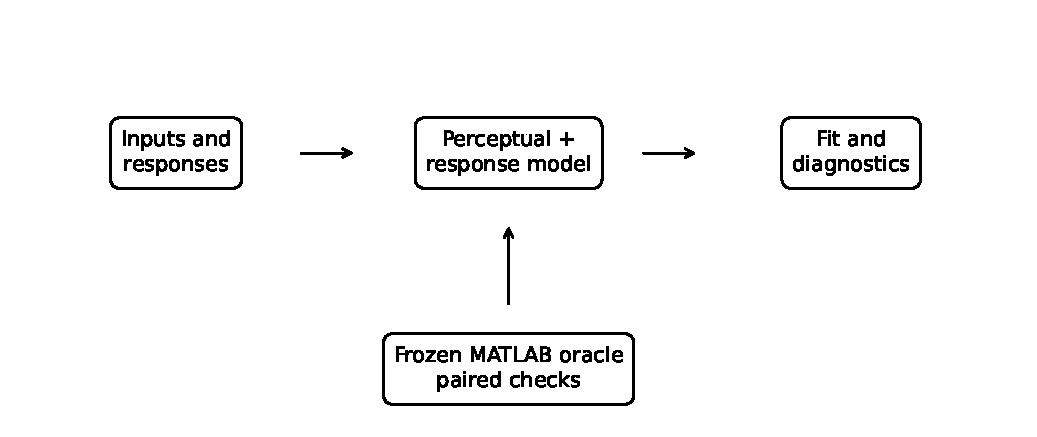
\includegraphics[width=\linewidth]{Fig1.pdf}
\captionof{figure}{User workflow and reference checks. Inputs and responses enter a configured perceptual/response pair, followed by fitting and inspection of trajectories, parameters and diagnostics. The separate frozen MATLAB oracle supplies paired evidence. This conceptual schematic contains no measured quantities}
\end{minipage}
\end{center}

\subsection{4 Evaluation methods}\label{evaluation-methods}

\subsubsection{4.1 Frozen scope and evidence
interpretation}\label{frozen-scope-and-evidence-interpretation}

All reported scientific results concern HGFX 1.0.0 and HGF Toolbox 8.2.0
at the identities in Supplement S1. The revision does not rerun recovery
experiments or modify frozen data, seeds, thresholds or failure
classifications. Existing machine-readable outputs are the basis of
tables and figures. New source inventories and presentation
transformations have their own manifests; they do not replace historical
artifacts.

The validation hierarchy starts with configuration and
transformed/native parameter semantics, then proceeds to numerical
primitives, fixed-parameter trajectories, trial likelihoods, objective
components, fitting and statistics, and complete workflows. This
ordering helps localize disagreement. A trajectory comparison can reveal
a first divergent trial, level and state before optimizer differences
obscure the cause. A fixed-vector objective check can distinguish a
response or prior mismatch from a fitting-path difference.
Fitted-parameter checks are meaningful only after these simpler
comparisons have a defensible common surface.

Four outcome classes are used. Direct parity means agreement under the
frozen criterion for a stated scope. A matched reference limitation
means that the oracle exhibits the corresponding instability or
limitation; it is not a scientific recovery success. A preserved failure
remains a failed criterion in the evidence record. A
not-directly-comparable quantity lacks a defensible common semantic or
numerical surface. These classifications are not interchangeable labels
for successful execution. In particular, product acceptance of a matched
limitation does not turn a failed inference experiment into a pass.

Numerical criteria are field-specific. The two official binary demo
workflows use 320 trials and compare release-relevant trajectories and
inference states at relative tolerance \(5\times10^{-11}\) and absolute
tolerance \(5\times10^{-13}\). Fitting, curvature and backend criteria
have their own scopes; a single tolerance is not applied across all
quantities. No criterion in this revision was relaxed to accommodate a
discrepancy. Correlation alone is insufficient because it can remain
high despite offsets, scaling changes or a small number of divergent
states.

\subsubsection{4.2 Paired recovery and model
selection}\label{paired-recovery-and-model-selection}

The paired recovery grid uses three binary perceptual models: classic,
enhanced and unbounded HGF. It includes truth scales of 0.15 and 0.35
prior standard deviations, trial counts of 128 and 256, and frozen
quasi-Newton settings. There are 72 parameter cases and 36
model-recovery datasets, with three candidate fits per model-recovery
dataset. Each model contributes 24 parameter cases, pooling two trial
counts, two truth scales and six replicates. Fits start once at resolved
transformed prior means, with at most 100 quasi-Newton iterations and no
random restarts. The three free parameters are omega2, omega3 and log
zeta (zero-based combined-vector positions 12, 13 and 14).

Predeclared scientific criteria are convergence rate at least 0.80,
median parameter-recovery correlation at least 0.50, median standardized
root mean square error (sRMSE) at most 1.00, and model-recovery balanced
accuracy at least 0.50. Parameter recovery asks how well fitted
parameters recover simulated truths. Model recovery asks whether model
selection recovers the generating model. Cross-implementation winner
agreement asks a third question: whether MATLAB and HGFX choose the same
candidate on the same data. Figure 3 separates the latter two quantities
visually.

For each transformed parameter, sRMSE is its root mean squared
estimation error divided by the population standard deviation of its
simulated truths across the 24 cases. The recorded implementation
substitutes a divisor of one only when that standard deviation is at
most \(10^{-12}\). Correlation is Pearson correlation across cases; the
reported median includes finite parameter correlations. Nonconverged but
returned fits remain in these metrics; an execution failure makes the
model summary incomplete. Convergence means termination at the argument
or gradient tolerance in HGFX. MATLAB convergence is inferred from the
retained iteration trace and absence of its
maximum-reset/maximum-iteration warnings, rather than from successful
function return. Supplement S2 gives parameter-wise results and the
selection confusion matrix. Historical failures remain archived
independently.

\subsubsection{4.3 Trial-horizon diagnostic
extension}\label{trial-horizon-diagnostic-extension}

A separate prospective experiment considered 128, 256, 512 and 1024
trials with the same three model families and frozen recovery criteria.
Its scientific comparison of 256 versus 1024 trials was conditional on a
paired-integrity gate. The shorter and intermediate horizons supplied
diagnostics. Invalid simulations and failed fits were retained rather
than redrawn. This design matters because selectively replacing invalid
cases could change the apparent relation between trial length and
recovery.

The integrity gate is logically prior to interpretation of horizon
trends. A promising recovery metric for one model or horizon does not
override disagreement between implementations elsewhere in the required
paired scope. The complete aggregate, diagnostic classifications and
provenance are provided in Supplement S3. The revision reports the
failed gate rather than treating executed shards as proof of a
successful scientific experiment.

\subsubsection{4.4 pyhgf comparison}\label{pyhgf-comparison}

The common-scope comparison pins pyhgf 0.3.2 and uses one fully
observed, fixed-parameter three-level binary HGF with 128 trials. Model
structure, update rules, initialization, parameters, input coding,
masks, precision and numerical guards were mapped before numerical
interpretation. The authorized settings include standard volatility
updates, mean-field updates, unit coupling, zero drift and native
inverse temperature 48. The comparison does not cover all pyhgf
networks, all HGFX families, parameter fitting or arbitrary response
models.

Mapped trajectory quantities use absolute tolerance \(10^{-10}\) and
relative tolerance \(10^{-8}\). The candidate response total negative
log-likelihood (NLL) surface uses absolute tolerance \(10^{-7}\) and
relative tolerance \(10^{-8}\). A response-probability boundary
nonfinite was prospectively assigned to the not-directly-comparable
class. It was not repaired after inspection by clipping probabilities.
The complete mapping and raw outputs make this limitation
distinguishable from a perceptual-trajectory mismatch.

\subsubsection{4.5 Backend evidence and published-study
feasibility}\label{backend-evidence-and-published-study-feasibility}

The backend comparison distinguishes compatibility CPU versus JAX CPU
from JAX CPU versus physical GPU. The first has a final-objective gap
criterion of 0.10; the second uses \(10^{-7}\). Retained physical-GPU
evidence comes from a recorded pre-release runtime with two visible
Tesla T4 devices, while the required fitting cells execute on one tested
device. Device enumeration and actual array residency are separate
checks. These measurements concern applicability and agreement, without
a speed or scaling hypothesis.

The empirical example follows the frozen toolbox's continuous-input
demonstration: a two-level classic HGF with the bayes\_optimal
likelihood evaluates the USD/CHF observations directly, with an empty
response vector. Default priors, placeholder resolution and optimizer
settings are retained. The complete sequence is used in its recorded
order, without generated responses or removed rows. It is a descriptive
fit to an empirical series, not an out-of-sample forecasting test.
Separate source audits of Pain 2025 (Lacombe-Thibault and Coll 2025) and
SPIRL (Hess et al. 2025) assess whether their customized participant
pipelines can be transferred without changing the models; neither
proceeds to fitting.

\subsubsection{4.6 Forward validation on published behavioral
inputs}\label{forward-validation-on-published-behavioral-inputs}

To evaluate fixed-parameter agreement on published behavioral inputs, we
used two 80-trial blocks or condition halves per participant prefix from
two archived behavioral input files (Reed et al. 2020; Suthaharan et al.
2021). The initial 326-block source check stopped before full-cohort
model execution because one Reed workspace variable was not a
participant identifier. The revised protocol, recorded before the paired
full-cohort execution, retained all 260 Suthaharan and 64 Reed blocks in
the two pinned source files. We preserved binary outcomes, three-choice
coding and the mask for trials with a missing choice or outcome. Both
implementations evaluated the same uncoupled three-arm perceptual model
at the native 17-parameter vector inherited from reference test M12B. We
compared 12 trajectory or inference-state outputs per block in CPU
binary64 with relative tolerance \(2\times10^{-9}\) and absolute
tolerance \(2\times10^{-11}\), including matched nonfinite values. The
workflow held all parameters fixed and omitted the observation model.
Supplement S7 records the source, protocol and software identities.

\subsection{5 Results}\label{results}

\subsubsection{5.1 Reference workflows and sensitive
fits}\label{reference-workflows-and-sensitive-fits}

The official workflow evidence supports scoped reproduction of the
binary enhanced-HGF and unbounded-HGF autoregressive workflows. In the
documented binary challenge regime, classic HGF encounters negative
posterior precision in both implementations while enhanced HGF
completes. Reproducing the expected failure is part of reference
behavior. It is not an improvement in the classic model, nor a reason to
conceal that case.

Two fitting cases retain endpoint or inference-equivalence failures and
are classified as matched reference limitations. The official stress fit
is sensitive to optimizer behavior within a numerical basin. The
separate fixed-seed holdout fit fails inference equivalence. Their
detailed paired records are in Supplement S2. Neither is summarized as
direct parameter parity. The core/API, sampling, analysis and Bayesian
parameter-averaging evidence concerns the documented release scope; it
is not a blanket assertion that all possible scientific workflows are
validated.

\begin{minipage}{\linewidth}
\textbf{Table 1.} Quantitative evidence and its boundaries. Each
criterion applies only to its stated surface. NR means a maximum
discrepancy was not retained in the classification artifact; it is not
zero

{\def\LTcaptype{none} % do not increment counter
\begin{tabular}{@{}
  >{\raggedright\arraybackslash}p{(\linewidth - 4\tabcolsep) * \real{0.3333}}
  >{\raggedright\arraybackslash}p{(\linewidth - 4\tabcolsep) * \real{0.3333}}
  >{\raggedright\arraybackslash}p{(\linewidth - 4\tabcolsep) * \real{0.3333}}@{}}
\toprule\noalign{}
\begin{minipage}[b]{\linewidth}\raggedright
Comparison and scope
\end{minipage} & \begin{minipage}[b]{\linewidth}\raggedright
Recorded measurement
\end{minipage} & \begin{minipage}[b]{\linewidth}\raggedright
Frozen criterion / interpretation
\end{minipage} \\
\midrule\noalign{}


Official binary eHGF challenge; 320 trials & No trajectory/state
mismatches; maximum NR & atol \(5\times10^{-13}\), rtol
\(5\times10^{-11}\); classic HGF fails in both \\
Official uHGF / AR1 workflow; 320 trials & No trajectory/state
mismatches; maximum NR & Same trajectory tolerances; two model paths \\
Sensitive eHGF fit; shared-state probe & Objective gap
\(2.84\times10^{-14}\); state gap zero & Endpoint mismatch preserved;
not fit parity \\
Paired binary model selection & 36/36 BIC winners agree & Exact winner
identity; recovery accuracy 0.583 \\
Mapped pyhgf perceptual comparison & 11 fields; maximum error
\(1.55\times10^{-15}\) & atol \(10^{-10}\), rtol \(10^{-8}\); one
128-trial case \\
Compatibility / JAX CPU fitting & Maximum objective gap 0.006784 &
Absolute gap \(\leq0.10\); four cells \\
JAX CPU / T4 fitting & Maximum objective gap \(1.42\times10^{-14}\) &
Absolute gap \(\leq10^{-7}\); four cells \\
\bottomrule
\end{tabular}
}
\end{minipage}


The trajectory checks, shared-state probe and fitted-objective checks
address different quantities. They do not certify arbitrary parameter
endpoints or custom study responses. The two sensitive fitting cases
remain matched reference limitations; their numerical localization is
summarized in Supplement S2.

The software comparison is deliberately asymmetric (Table 2). The MATLAB
package is the specification used for this evaluation, HGFX is evaluated
as its scoped reimplementation, and pyhgf is compared only after
establishing a common surface. Thus a row marked untested describes the
limits of this study rather than an absent software capability. Runtime
requirements and model semantics should be considered separately:
sharing a language or accelerator framework does not make likelihoods or
fitted statistics interchangeable. Likewise, retaining MATLAB-style
aliases is useful for migration, but interface similarity is weaker
evidence than agreement of transformed parameters and objective
components. The same rule applies to customized published studies, where
familiar perceptual model names can accompany materially different
response definitions.

\begin{minipage}{\linewidth}
\textbf{Table 2.} Version-bound software comparison. Sources are the
frozen oracle, release configuration/API evidence, and the prospective
pyhgf semantic mapping. Untested does not mean unsupported

{\def\LTcaptype{none} % do not increment counter
\begin{tabular}{@{}
  >{\raggedright\arraybackslash}p{(\linewidth - 6\tabcolsep) * \real{0.2500}}
  >{\raggedright\arraybackslash}p{(\linewidth - 6\tabcolsep) * \real{0.2500}}
  >{\raggedright\arraybackslash}p{(\linewidth - 6\tabcolsep) * \real{0.2500}}
  >{\raggedright\arraybackslash}p{(\linewidth - 6\tabcolsep) * \real{0.2500}}@{}}
\toprule\noalign{}
\begin{minipage}[b]{\linewidth}\raggedright
Property
\end{minipage} & \begin{minipage}[b]{\linewidth}\raggedright
MATLAB HGF 8.2.0
\end{minipage} & \begin{minipage}[b]{\linewidth}\raggedright
HGFX 1.0.0
\end{minipage} & \begin{minipage}[b]{\linewidth}\raggedright
pyhgf 0.3.2
\end{minipage} \\
\midrule\noalign{}


Role here & Frozen reference & Reference-compatible Python
implementation & Common-scope comparator \\
User runtime & MATLAB & Python/NumPy/JAX; no MATLAB & Python/JAX \\
Configuration semantics & Specification & Tested configured surfaces &
Mapped in one binary case \\
Inference & Reference approximate updates & Documented HGF/eHGF/uHGF
families & Network-based construction; one mapped cell tested \\
Fitting comparison here & Paired oracle fits & Direct/limited results
retained & Untested \\
Accelerator evidence here & Untested & Retained T4 objective cells &
Untested \\
Response NLL comparison & Reference in paired HGFX scope & Case-specific
& NDC in common-scope cell \\
\bottomrule
\end{tabular}
}
\end{minipage}


\subsubsection{5.2 Recovery and implementation
agreement}\label{recovery-and-implementation-agreement}

Parameter-recovery criteria are not fully met in the paired grid (Table
3 and Figure 2). Classic and enhanced HGF fail the correlation and sRMSE
criteria. Unbounded HGF also fails the convergence criterion. The
corresponding MATLAB and HGFX metrics are close, which supports the
narrow matched-limitation interpretation; it does not establish that
those parameters can be estimated adequately in the tested designs.

\begin{minipage}{\linewidth}
\textbf{Table 3.} Paired parameter recovery across both truth scales.
Entries are MATLAB/HGFX; displayed values are rounded from
full-precision artifacts. Each model contributes 24 parameter cases.
Thresholds: convergence \textgreater=0.80, median correlation
\textgreater=0.50, median sRMSE \textless=1.00

{\def\LTcaptype{none} % do not increment counter
\begin{tabular}{@{}
  >{\raggedright\arraybackslash}p{(\linewidth - 8\tabcolsep) * \real{0.2000}}
  >{\raggedright\arraybackslash}p{(\linewidth - 8\tabcolsep) * \real{0.2000}}
  >{\raggedright\arraybackslash}p{(\linewidth - 8\tabcolsep) * \real{0.2000}}
  >{\raggedright\arraybackslash}p{(\linewidth - 8\tabcolsep) * \real{0.2000}}
  >{\raggedright\arraybackslash}p{(\linewidth - 8\tabcolsep) * \real{0.2000}}@{}}
\toprule\noalign{}
\begin{minipage}[b]{\linewidth}\raggedright
Model
\end{minipage} & \begin{minipage}[b]{\linewidth}\raggedright
Convergence
\end{minipage} & \begin{minipage}[b]{\linewidth}\raggedright
Median correlation
\end{minipage} & \begin{minipage}[b]{\linewidth}\raggedright
Median sRMSE
\end{minipage} & \begin{minipage}[b]{\linewidth}\raggedright
Failed criteria
\end{minipage} \\
\midrule\noalign{}


Classic HGF & 0.833/0.833 & 0.203/0.203 & 2.610/2.610 & Correlation,
sRMSE \\
Enhanced HGF & 0.917/0.917 & 0.462/0.462 & 2.359/2.359 & Correlation,
sRMSE \\
Unbounded HGF & 0.792/0.792 & 0.381/0.381 & 2.958/2.958 & All three \\
\bottomrule
\end{tabular}
}
\end{minipage}


\begin{center}
\begin{minipage}{\linewidth}
\centering
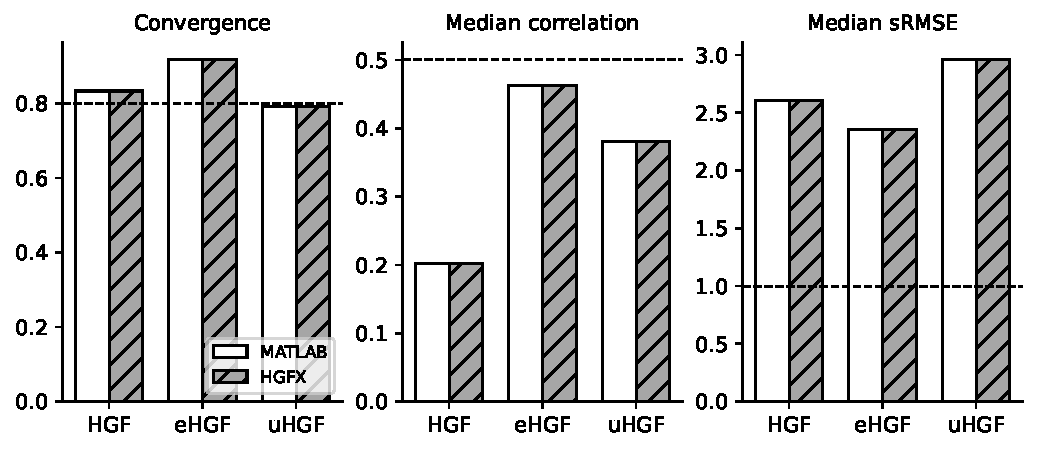
\includegraphics[width=\linewidth]{Fig2.pdf}
\captionof{figure}{Paired parameter-recovery summaries for the frozen grid, with the predeclared thresholds shown as dashed lines. These are descriptive aggregate metrics without error bars, not a scientific recovery pass. All three model families retain failed criteria}
\end{minipage}
\end{center}

All 36 model-recovery datasets have the same minimum-BIC winner in
MATLAB and HGFX (Figure 3a). Generating-model recovery balanced accuracy
is 0.5833333333333334 for both (Figure 3b). The perfect implementation
agreement and imperfect generating-model recovery coexist because they
measure different properties. The recovery threshold applies to balanced
accuracy, not to cross-implementation agreement. This result supports
reproducibility of the tested selection behavior, not universal
discrimination among HGF families.

\begin{center}
\begin{minipage}{\linewidth}
\centering
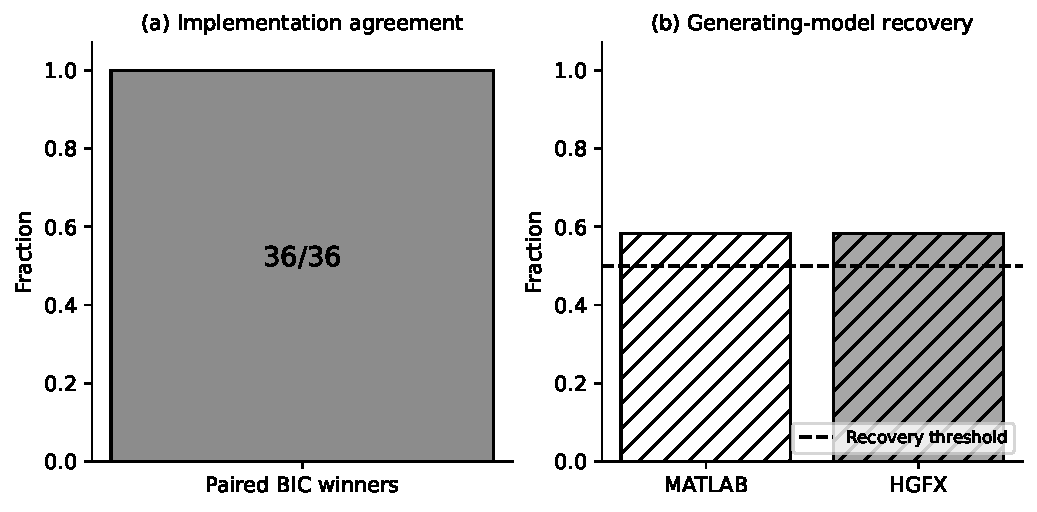
\includegraphics[width=\linewidth]{Fig3.pdf}
\captionof{figure}{Implementation agreement and generating-model recovery in the same 36 paired datasets, with three candidate models each. Panel (a) shows 36/36 matching BIC winners. Panel (b) shows balanced accuracy of 0.583 for each implementation; only this panel includes the frozen recovery threshold of 0.50. Bars are deterministic summaries of the frozen grid, without error bars}
\end{minipage}
\end{center}

\subsubsection{5.3 Trial horizon, software comparison and
backends}\label{trial-horizon-software-comparison-and-backends}

The trial-horizon experiment fails its paired-integrity gate. A
retrospective audit of the original 24 shard archives clarifies why: all
62 datasets with nonempty selected-model labels agree, while ten
datasets have no selected model in either implementation because
simulation was invalid. The frozen checker counts these empty pairs as
failed winner matches; they are not ten pairs choosing different models.
Of 144 parameter cases, 20 share an invalid simulation and four have an
HGFX initial-objective rejection with a MATLAB success flag. Two of
those MATLAB outputs have nonfinite negative log joint values; the other
two return finite values. All 120 successful pairs have the expected
free indices. Thus the 24 failed index checks reflect empty failure
outputs, not observed parameter-order differences between successful
fits. The classifier propagates its global gate failure to all three
families, so its labels do not localize a defect to every family. These
distinctions correct interpretation without changing the frozen gate,
replacing failed data or claiming identifiability. Supplement S3 retains
the four asymmetric cases and the limits of their localization.

All 11 mapped perceptual quantities pass the common-scope pyhgf
criteria. Maximum absolute differences range from approximately
\(1.11\times10^{-16}\) to \(1.55\times10^{-15}\) in the frozen cell.
Participant-response NLL is NDC: the power-ratio transformation on the
pyhgf side reaches an exact probability boundary for the recorded
inverse temperature, yielding a nonfinite comparison surface. This
outcome limits a response comparison while leaving the mapped perceptual
agreement intact. Figure 4 shows overlapping trajectories; the
field-wise error record in the supplement is necessary to interpret that
overlap.

\begin{center}
\begin{minipage}{\linewidth}
\centering
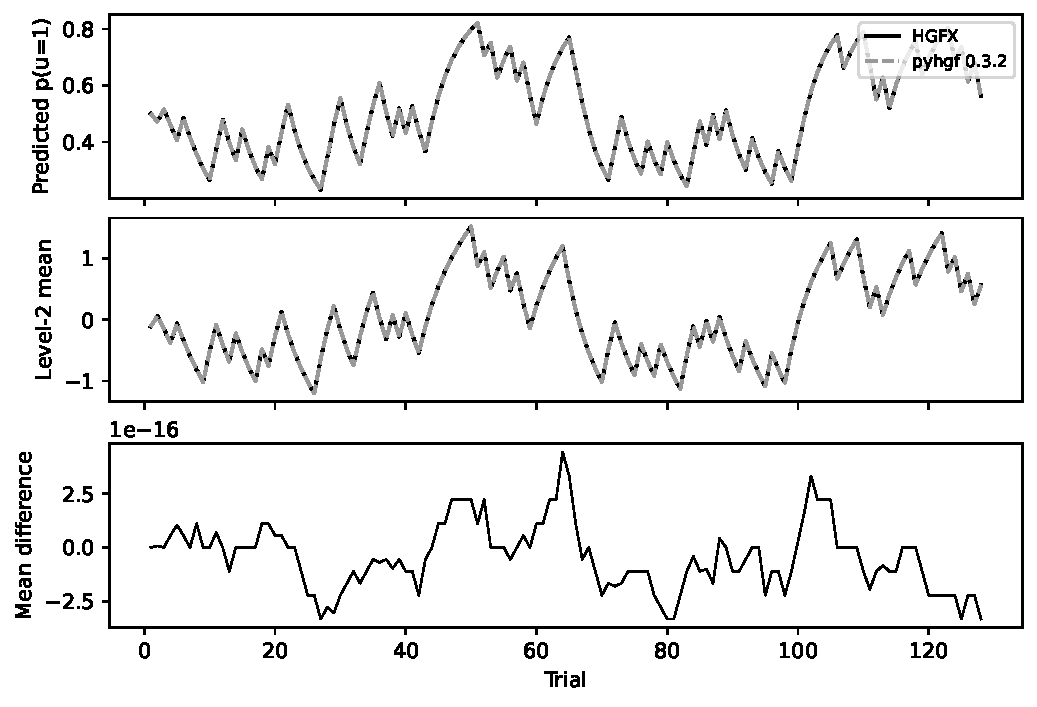
\includegraphics[width=\linewidth]{Fig4.pdf}
\captionof{figure}{HGFX and pyhgf 0.3.2 trajectories in the single authorized 128-trial binary-HGF case. Solid and dashed lines distinguish implementations. The first two panels show predicted input probability and level-2 posterior mean; the third shows the signed HGFX-minus-pyhgf level-2 mean difference over all trials. Eleven mapped perceptual quantities pass their criteria. Participant-response NLL remains NDC. No uncertainty bands are shown because these are deterministic fixed-parameter trajectories}
\end{minipage}
\end{center}

The compatibility-versus-JAX CPU maximum final-objective gap is
0.006783711260709424 against its 0.10 criterion. The four retained
CPU-versus-T4 fitting cells pass their \(10^{-7}\) criterion, with
maximum gap \(1.4210854715202004\times10^{-14}\). Figure S2 expresses
each gap relative to its own threshold. The retained GPU runtime and
source identity are provided in Supplement S4. These are different
comparisons with different criteria; their gap magnitudes should not be
read as a ranking of hardware accuracy.

\subsubsection{5.4 Empirical-input workflow and application
boundary}\label{empirical-input-workflow-and-application-boundary}

The continuous-input example applies the released wheel to the entire
USD/CHF series distributed with the frozen toolbox. The upstream demo
describes exchange rates during 2010 and 2011; the file supplies values
without calendar labels. Consequently, the example uses observation
number rather than invented dates and treats the series' upstream
description as its provenance. It estimates perceptual parameters from
the input likelihood, without participant choices or synthetic response
measurements. The run completed in 182 seconds on CPU float64, returning
negative log likelihood -2387.622 and BIC -4736.724 for 614
observations. A continuous density can exceed one, so a negative
negative-log-likelihood is not itself an error. Figure 5 shows the
observations and fitted-filter predictions. Parameters were estimated
from the full series: the one-step predictions are therefore in-sample
diagnostics, not held-out forecasts. Numerical-derivative warnings
occurred; finite statistics are not treated as a convergence or
curvature-validation certificate. Supplement S6 records the execution
and remaining diagnostics.

The example shows how an analyst can inspect one-step predictions and
changing latent volatility using a standard configuration. It does not
establish financial forecasting performance or reproduce a participant
study. Pain's custom response permissions and historical environment
remain unresolved. SPIRL requires a separately validated custom
perceptual model and seven joint choice/response-time models. The source
audits identify those boundaries; their file-acquisition details belong
to the reproducibility dossier, not to an empirical result.

\begin{center}
\begin{minipage}{\linewidth}
\centering
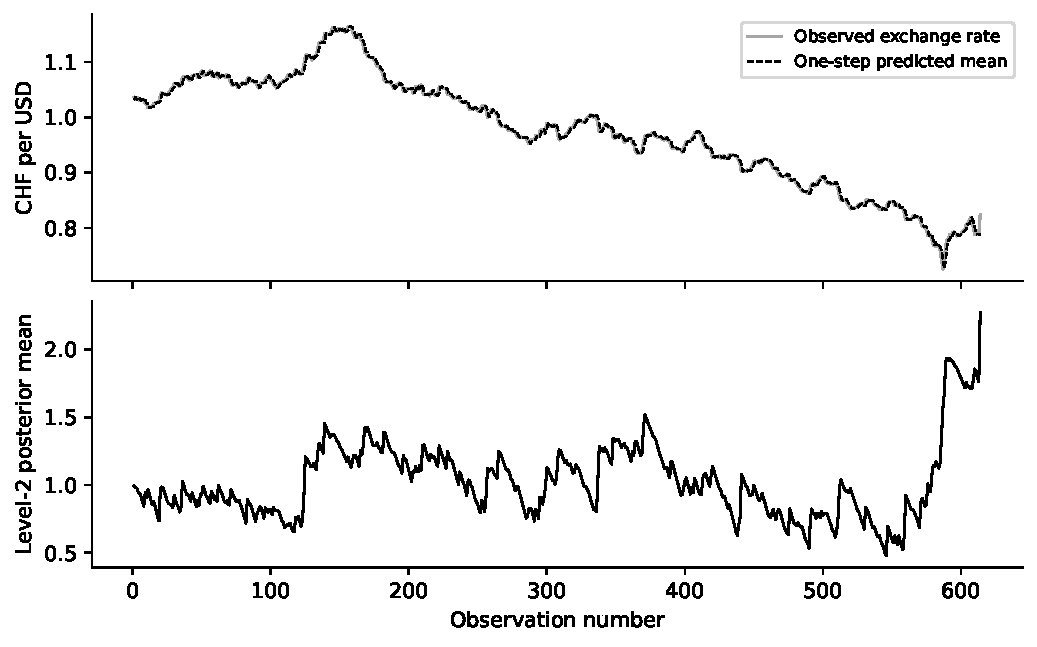
\includegraphics[width=\linewidth]{Fig5.pdf}
\captionof{figure}{Empirical-input worked example with all 614 USD/CHF observations from the frozen toolbox demo. The upper panel shows observed rates and one-step predicted means from the continuous two-level HGF; the lower panel shows the fitted level-2 posterior mean, which modulates innovation variance. Parameters are estimated using the full series. No held-out accuracy, parameter uncertainty, new MATLAB agreement or participant-study replication is implied}
\end{minipage}
\end{center}

\subsubsection{5.5 Forward agreement on published behavioral
inputs}\label{forward-agreement-on-published-behavioral-inputs}

Both implementations completed the fixed-parameter comparison for all
324 blocks (25,920 input trials). Across 3,888 fields and 2,540,160
compared array entries, no entry exceeded the specified criterion. The
largest absolute difference among finite pairs was
\(3.109\times10^{-15}\). Python emitted warnings in 48 of the 324
blocks. The archived summary retains the warning counts, and the warning
mechanisms remain uncharacterized. The result concerns numerical
compatibility of the perceptual filter on the two selected input files.
Replication of the original fitted parameters, model comparisons and
group-level results remains outside this experiment.

\subsection{6 Discussion}\label{discussion}

HGFX serves analysts who need the tested conventions of a particular
MATLAB HGF release in a Python environment. The contribution is the
combination of a usable interface and scoped numerical evidence:
parameter spaces, priors, masks, likelihoods and returned statistics are
part of the analysis specification. Table 1 separates this evidence into
surfaces that a user can evaluate before transporting an existing
workflow. A shared model name alone is insufficient.

Implementation agreement and scientific recovery answer different
questions. In the paired grid, 36 matching BIC winners coexist with
generating-model balanced accuracy of 0.583. Parameter-wise results
further show that the median recovery summary conceals substantial
heterogeneity: classic HGF recovers omega2 well in this grid, while its
omega3 correlation is negative. This does not establish universal
failure or success of either parameter. The narrow truth ranges, pooled
horizons, observation model and single-start fitting constrain the
result. Individual-difference studies need recovery assessment for their
own design.

The horizon audit also illustrates why failure labels require inspection
of raw outputs. Missing winners after invalid generation are different
from competing finite model selections. Empty index arrays after
execution failure are different from reordered parameters. Nonetheless,
four asymmetric initial-fit outcomes remain, and the historical outputs
do not identify their first divergent trial, level and intermediate
state. The extended horizon grid therefore remains outside the supported
paired-fitting claim. No general structural-identifiability conclusion
follows, and the successful subset does not rescue the original gate.

The published behavioral inputs test the same perceptual calculation
across observed choice and outcome sequences from two source files.
Their numerical agreement extends the synthetic checks to those inputs
at one parameter vector. Assessing transportability of the original
analyses would require their observation likelihoods, priors,
optimization procedures, sample definitions and outcome analyses. The 48
blocks with Python warnings also warrant diagnostic follow-up. The
USD/CHF example separately demonstrates fitting for a standard
continuous model, while the Pain and SPIRL audits identify open
requirements for customized workflows.

A separate untimed diagnostic on 64 synthetic standard-binary HGF
datasets further distinguishes forward agreement from complete-fit
agreement. Sixty-three fits met the existing full-output criteria. For
subject index 7, four level-2 posterior means and four corresponding
predicted means exceeded the trajectory criterion, although the fitted
parameters and other compared fit quantities met their field-specific
criteria. This cohort result limits an end-to-end fitting-equivalence
claim. It also motivates comparison of complete fitted trajectories
after checking the fixed-parameter calculation. The
\href{https://github.com/ahmadkhanloo/hgfx/blob/81d9e8fc67c1d801f7d749cf44ba9fcfffdbf1f3/benchmarks/runtime_v1/fit_cohort_results/summary-41863441006.json}{archived
64-fit record} retains the failed values and unchanged thresholds.

HGFX and pyhgf have complementary evaluation scopes here. Eleven mapped
perceptual quantities agree at rounding scale in one case, but the
response-probability boundary prevents a likelihood-equivalence claim.
Likewise, T4 objective agreement does not establish throughput or
scaling. Broader response comparisons and performance benchmarks require
their own prospective protocols.

Compatibility is tied to the immutable 8.2.0 reference and the tested
scopes, not future releases or arbitrary custom models. Two sensitive
fitting cases remain exact-scope reference limitations; the horizon
failures remain unresolved beyond the recorded diagnostic stages. Within
those boundaries, the package makes established HGF workflows accessible
without MATLAB at user runtime and gives analysts explicit evidence for
deciding what can be transferred and what still requires validation.

\subsection{7 Data and code
availability}\label{data-and-code-availability}

HGFX 1.0.0 is available from the
\href{https://github.com/ahmadkhanloo/hgfx/releases/tag/v1.0.0}{versioned
release} (HGFX developers 2026) under the MIT license. The repository
provides the manuscript, evidence manifests and reproducibility
instructions. Supplement S7 identifies the original behavioral input
files and their source commits, the preparation and comparison code, and
the archived numerical summary. Participant inputs and per-trial
trajectories are available only through their respective original
sources or regeneration under the recorded workflow, as applicable. They
are excluded from this package. MATLAB is required to regenerate the
reference outputs.

\subsection{Electronic supplementary material}

Online Resource 1 (ESM\_1.pdf) contains frozen identities, numerical validation and recovery details, trial-horizon diagnostics, backend and comparator evidence, published-input source provenance, and the bounded warning and feasibility follow-up.

\subsection{Statements and
Declarations}\label{statements-and-declarations}

\subsubsection{Funding and competing
interests}\label{funding-and-competing-interests}

No specific grant funding was received for this work. Mohammad
Ahmadkhanloo is the developer and maintainer of HGFX and declares no
other competing interests.

\subsubsection{Author contributions and
ethics}\label{author-contributions-and-ethics}

Mohammad Ahmadkhanloo: conceptualization, software, validation, formal
analysis, data curation, visualization, and writing (original draft and
review/editing). The software evaluation uses existing publicly archived
choice and outcome sequences as numerical inputs and includes an
empirical exchange-rate example. It involved no new participant
recruitment or data collection. The source studies report their original
ethics and consent procedures (Reed et al. 2020; Suthaharan et al.
2021).

\subsubsection{Generative AI use and
accountability}\label{generative-ai-use-and-accountability}

OpenAI ChatGPT assisted with source inventory, code and test drafting,
manuscript restructuring and substantial prose generation, figure
preparation, and package checks. This work extends beyond copyediting.
Automated source checks and editorial review are recorded as such, not
as completed human verification. The author confirmed authorship and
declarations and remains responsible for verification and approval of
the final scientific content before submission.

\section*{References}\label{bibliography}
\addcontentsline{toc}{section}{References}

\protect\phantomsection\label{refs}
\begin{CSLReferences}{1}{1}
\interlinepenalty=10000
\bibitem[\citeproctext]{ref-jax2018github}
Bradbury J, Frostig R, Hawkins P, et al (2018)
\href{https://github.com/jax-ml/jax}{{JAX}: Composable transformations
of {Python}+{NumPy} programs}

\bibitem[\citeproctext]{ref-diaconescu2014}
Diaconescu AO, Mathys C, Weber LAE, et al (2014) Inferring on the
intentions of others by hierarchical {Bayesian} learning. PLOS
Computational Biology 10:e1003810.
\url{https://doi.org/10.1371/journal.pcbi.1003810}

\bibitem[\citeproctext]{ref-fraessle2021tapas}
Frässle S, Aponte EA, Bollmann S, et al (2021) {TAPAS}: An open-source
software package for translational neuromodeling and computational
psychiatry. Frontiers in Psychiatry 12:680811.
\url{https://doi.org/10.3389/fpsyt.2021.680811}

\bibitem[\citeproctext]{ref-frostig2018}
Frostig R, Johnson MJ, Leary C (2018) Compiling machine learning
programs via high-level tracing. In: Proceedings of SysML

\bibitem[\citeproctext]{ref-spirl_2025}
Hess AJ, Iglesias S, Köchli L, et al (2025) Bayesian workflow for
generative modeling in computational psychiatry. Computational
Psychiatry. \url{https://doi.org/10.5334/cpsy.116}

\bibitem[\citeproctext]{ref-hgfx100}
HGFX developers (2026)
\href{https://github.com/ahmadkhanloo/hgfx}{{HGFX}: A {GPU}-native
{Python} toolbox for hierarchical {Gaussian} filters}

\bibitem[\citeproctext]{ref-iglesias2013}
Iglesias S, Mathys C, Brodersen KH, et al (2013) Hierarchical prediction
errors in midbrain and basal forebrain during sensory learning. Neuron
80:519--530. \url{https://doi.org/10.1016/j.neuron.2013.09.009}

\bibitem[\citeproctext]{ref-pain_2025}
Lacombe-Thibault M, Coll M-P (2025) Expectations and uncertainty shape
pain perception during learning. The Journal of Pain.
\url{https://doi.org/10.1016/j.jpain.2025.105569}

\bibitem[\citeproctext]{ref-legrand2026pyhgf}
Legrand N, Weber L, Waade PT, et al (2026) Pyhgf: A neural network
library for predictive coding. PLOS Computational Biology 22:e1014340.
\url{https://doi.org/10.1371/journal.pcbi.1014340}

\bibitem[\citeproctext]{ref-mathys2011}
Mathys C, Daunizeau J, Friston KJ, Stephan KE (2011) A {Bayesian}
foundation for individual learning under uncertainty. Frontiers in Human
Neuroscience 5:39. \url{https://doi.org/10.3389/fnhum.2011.00039}

\bibitem[\citeproctext]{ref-mathys2014}
Mathys CD, Lomakina EI, Daunizeau J, et al (2014) Uncertainty in
perception and the hierarchical {Gaussian} filter. Frontiers in Human
Neuroscience 8:825. \url{https://doi.org/10.3389/fnhum.2014.00825}

\bibitem[\citeproctext]{ref-peng2011reproducible}
Peng RD (2011) Reproducible research in computational science. Science
334:1226--1227. \url{https://doi.org/10.1126/science.1213847}

\bibitem[\citeproctext]{ref-reed2020}
Reed EJ, Uddenberg S, Suthaharan P, et al (2020) Paranoia as a deficit
in non-social belief updating. eLife 9:e56345.
\url{https://doi.org/10.7554/eLife.56345}

\bibitem[\citeproctext]{ref-suthaharan2021}
Suthaharan P, Reed EJ, Leptourgos P, et al (2021) Paranoia and belief
updating during the {COVID-19} crisis. Nature Human Behaviour
5:1190--1202. \url{https://doi.org/10.1038/s41562-021-01176-8}

\bibitem[\citeproctext]{ref-wilson2019ten}
Wilson RC, Collins AGE (2019) Ten simple rules for the computational
modeling of behavioral data. eLife 8:e49547.
\url{https://doi.org/10.7554/eLife.49547}

\end{CSLReferences}

\end{document}
